\subsection{Inception Score (IS) and Frechet Inception Distance
(FID)}

Both the Inception Score (or IS) and the Frechet Inception Distance (or
FID) are metrics to assess the quality of images generated by a GAN.

\subsubsection{Generated data}

To calculate the Inception Score and the Frechet Inception Distance, we
are going to use some generated samples from the previous exercise. The
\lstinline{samples.pickle} contains 800 samples recorded
over 50 epochs (16 samples per epoch). We can visualize them below. The
samples are saved as \lstinline{np.array} and contain
images in the {[}0, 255{]} range.

\begin{lstlisting}[language=Python]
# run this cell once to install the dependency
# you will have to restart the kernel afterwards
!pip install ipywidgets
\end{lstlisting}

\begin{lstlisting}[language=Python]
import pickle
from typing import List

import matplotlib.pyplot as plt
import numpy as np
\end{lstlisting}

\begin{lstlisting}[language=Python]
# helper function for visualization.

def view_samples(epoch: int, samples: List[np.array]):
    fig, axes = plt.subplots(figsize=(14,4), nrows=2, ncols=8, sharey=True, sharex=True)
    for ax, img in zip(axes.flatten(), samples[16 * epoch: 16 * (epoch + 1)]):
        ax.xaxis.set_visible(False)
        ax.yaxis.set_visible(False)
        im = ax.imshow(img.reshape((32,32,3)))
    plt.show()
\end{lstlisting}

\begin{lstlisting}[language=Python]
with open('../samples.pkl', 'rb') as f:
    samples = pickle.load(f)
\end{lstlisting}

\begin{lstlisting}[language=Python]
view_samples(49, samples)
\end{lstlisting}

\subsubsection{Inception score}

The Inception Score was introduced by the
\href{https://arxiv.org/pdf/1606.03498.pdf}{Improved Techniques for
Training GANs} paper. This metric relies on the following approach: 
\begin{itemize}
    \item generated images are fed through the \href{https://arxiv.org/pdf/1409.4842.pdf}{Inception model} pretrained on the ImageNet dataset
    \item the probability distribution for each image should have \href{https://en.wikipedia.org/wiki/Entropy_(information_theory)}{low-entropy}. In other words, the model should output high probabilities for a single class and be confident that the image contains one object. We call this distribution the \textbf{conditional label distribution}.
    \item the probability distribution of all the classes over the whole dataset should have high entropy, meaning that the generative model creates images with high variability. We call this distribution the \textbf{marginal distribution}.
\end{itemize}
The inception score is calculated using the
\href{https://en.wikipedia.org/wiki/Kullback\%E2\%80\%93Leibler_divergence}{Kullback--Leibler
Divergence} (KL Divergence).

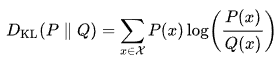
\includegraphics[width=1\linewidth]{img//genAdvNet//deepGAN/kl_divergence.png}

The KL divergence is a measure of how two distributions are similar.
Since we want the conditional label distribution to have
\href{https://en.wikipedia.org/wiki/Entropy_(information_theory)}{low
entropy} (think of a very low spread gaussian for example) and the
marginal distribution to have high entropy (think uniform distribution),
we want to \textbf{maximize the KL divergence}.

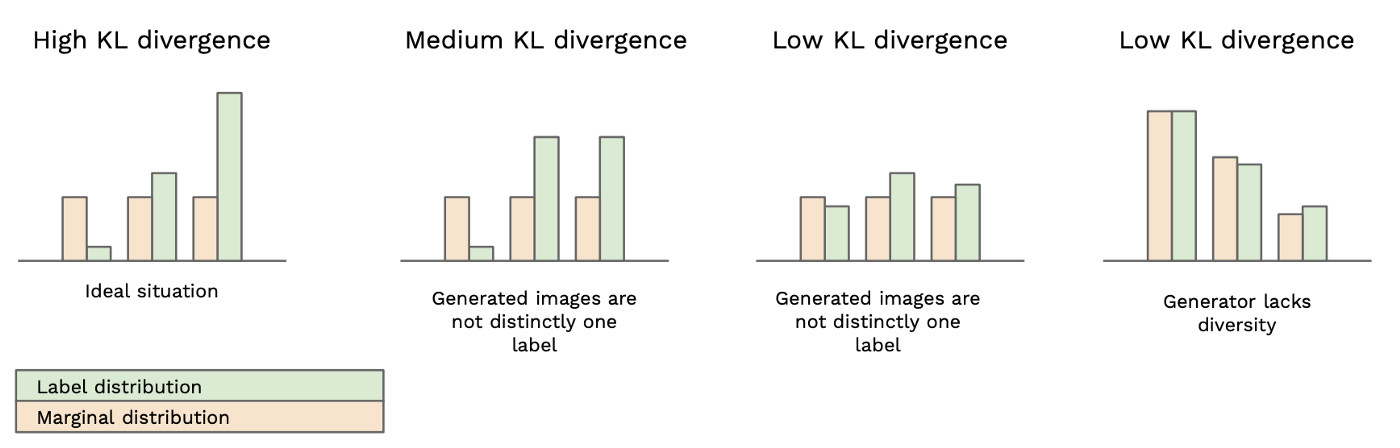
\includegraphics[width=1\linewidth]{img//genAdvNet//deepGAN/fid_score.png}

\href{https://medium.com/octavian-ai/a-simple-explanation-of-the-inception-score-372dff6a8c7a}{This article} explains the inception score in great depth.

\paragraph{Tips:}

\begin{itemize}
\item the \lstinline{inception_v3} pytorch model outputs the logits, not the probability and you will need to use the softmax activation to get probabilities.
\item look at the \href{https://docs.scipy.org/doc/scipy/reference/generated/scipy.stats.entropy.html}{scipy.stats.entropy}
  function for the kl divergence calculation.
\item you can find the pytorch Inception\_v3 model \href{https://pytorch.org/hub/pytorch_vision_inception_v3/}{here}. Don't forget to reshape the inputs!
\item if you are stuck, you can find the pytorch implementation of the inception score from the authors of the paper \href{https://github.com/openai/improved-gan/blob/master/inception_score/model.py}{here}.
\end{itemize}

\paragraph{Notes:}
In the original paper, they recommend to use 10 splits and calculate the mean and standard deviation of the score over the 10 splits. They also recommend to use large datasets (over 50k images). Here, we are using a small dataset and therefore will not take the split approach.

\begin{lstlisting}[language=Python]
import torch
from PIL import Image
from torchvision import transforms
from torchvision.models.inception import inception_v3
from scipy.stats import entropy
\end{lstlisting}

\begin{lstlisting}[language=Python]
def calculate_scores(samples: List[np.ndarray]) -> List[np.ndarray]:
    """
    This function calculates the score for each sample.
    """
    # load model
    inception_model = inception_v3(pretrained=True, transform_input=False)
    inception_model.eval()
    inception_model.cuda()
    
    # preprocessing
    preprocess = transforms.Compose([
        transforms.Resize(299),
        transforms.CenterCrop(299),
        transforms.ToTensor(),
        transforms.Normalize(mean=[0.485, 0.456, 0.406], std=[0.229, 0.224, 0.225]),
    ])    
    
    # forward pass
    scores = []
    for image in samples:
        image = Image.fromarray(image)
        input_tensor = preprocess(image)
        input_batch = input_tensor.unsqueeze(0).cuda()
        output = inception_model(input_batch)
        probs = torch.nn.functional.softmax(output[0].cpu().detach(), dim=0)
        scores.append(probs.numpy())
    return scores
\end{lstlisting}

\begin{lstlisting}[language=Python]
scores = calculate_scores(samples)
\end{lstlisting}

\begin{lstlisting}[language=Python]
def get_inception_score(scores: List[np.ndarray]) -> float:
    total_scores = []
    py = np.mean(scores, axis=0)

    # calculate the kl divergence
    kl = []
    for pyx in scores:
        ent = entropy(pyx, py)
        kl.append(ent)
    return np.exp(np.mean(kl))
\end{lstlisting}

\begin{lstlisting}[language=Python]
inception_score = get_inception_score(scores)
print(inception_score)
\end{lstlisting}

\subsubsection{Frechet Inception Distance}

The Frechet Inception Distance was first introduced by the
\href{https://arxiv.org/pdf/1706.08500.pdf}{GANs Trained by a Two
Time-Scale Update Rule Converge to a Local Nash Equilibrium} paper. \newline

The Inception Score was a groundbreaking metric for measure GAN
performances but it has a major flaw: \textbf{it does not take into
account the statistics of the ``real'' dataset the GAN is supposed to
mimic and only uses the generated images.} \newline

The FID takes a different approach: 
\begin{itemize}
    \item for each image in the generated dataset \textbf{and} the target (real) dataset, get the latent representation by running the Inception model. The latent representation of each image is the output of the penultimate layer, before the final classification layer.
    \item calculate the mean and the covariance of the real distribution (\(m_{r}\) and \(C_{r}\))
    \item calculate the mean and the covariance of the generated distribution (\(m_{g}\) and \(C_{g}\))
    \item calculate the Frechet Distance defined below:
\end{itemize}

\(FID = ||m_{r} - m_{g}||^{2}_{2} + Tr(C_{r}) + Tr(C_{g}) - 2 Tr(C_{r}C_{g})^{1/2}\)

where \(||.||_{2}\) is the L-2 norm and \(Tr\) the trace of the
covariance matrices. \newline

In this exercise, we will simply ask you to implement the FID
calculation, assuming that you already have calculated the mean and
covariance of both distribution.

\paragraph{Tips:}
\begin{itemize}
\item you can calculate the trace of the covariance matrices using \lstinline{np.trace}
\end{itemize}

\begin{lstlisting}[language=Python]
from scipy import linalg
\end{lstlisting}

\begin{lstlisting}[language=Python]
def get_fid(mu1: np.array, sigma1: np.array, mu2: np.array, sigma2: np.array):
    """
    Calculate the FID. 
    """
    diff = mu1 - mu2
    
    # calculate the square root of the dot product of the covariance matrices
    covmean, _ = linalg.sqrtm(sigma1.dot(sigma2), disp=False)
    
    # calculate the trace
    tr_covmean = np.trace(covmean)

    return (diff.dot(diff) + np.trace(sigma1)
            + np.trace(sigma2) - 2 * tr_covmean)
\end{lstlisting}

\begin{lstlisting}[language=Python]
samples1 = np.random.randn(100, 2048)
mu1 = np.mean(samples1, axis=0)
sigma1 = np.cov(samples1)

samples2 = np.random.randn(100, 2048)
mu2 = np.mean(samples2, axis=0)
sigma2 = np.cov(samples2)
\end{lstlisting}

\begin{lstlisting}[language=Python]
fid = get_fid(mu1, sigma1, mu2, sigma2)
print(fid)
\end{lstlisting}
